%%%%%% BACKGROUND %%%%%%
\newpage
\section{Bipolar disorder}

Bipolar disorder is the disorder where you experience extreme mood swings. One day you can feel amazing and 
everything is fine, but the next day you feel like you don't belong anywhere in this universe. 
Mood swings in general is not something that you should be concerned about. It is however the extreme cases where 
your mind turns 180 degrees from day to day that is the main symptom of bipolar disorder. 
There is not really a specific type of people that get this; they can be of any age and any gender, 
but most people that suffer from it find out (by having an experience or episode) around age 25 \cite{bipolar_statistics}. 

When talking about bipolar disorder, we often separate between the states \emph{normal}, \emph{mania} 
and \emph{depression}. The last two are the states we usually talk about, since a normal state isn't that interesting. 
These two states are very different, but they have some similarities, for example sleeping problems. 

When a bipolar person is in a manic state, he/she may do things that they never would have intended doing, 
like spending a lot of money on items they really don't need, or abusing drugs/alcohol. 
They may also feel really excited or powerful \cite{bipolar_overview}. 

A bipolar patient is in a depressive state when he or she is in a bad mood swing. They can stop doing everything 
they usually like to do, and lie down in bed all day with no motivation to do anything useful. 
They may feel useless and that they don't belong here, or being guilty of something they may or may not have done. 
In some cases, a depression may even end up with suicidality, where the person either just thinks of death, 
or actually attempt suicide (actually 20\% of people diagnosed with bipolarity commit suicide \cite{bipolar_statistics}). 

The frequency of these symptoms can vary. One year they can have these mood swings every day for several weeks at the time, 
and the next they get them less frequent, like once every month. 

We also separate between bipolar disorder type I and II, with the main difference being that the manic episodes 
are way more aggressive in type I \cite{bipolar_types}.

Statistics say that bipolarity is genetically inheritable, with 23\% chance of getting a child with bipolar disorder 
if one parent is bipolar, and 66\% if both parents are \cite{bipolar_statistics}. 

%% Use stories from book?

\newpage
\section{Machine learning}
Machine learning is the field of computer science where you basically throw a lot of data into an algorithm
and expect it to give you answers to whatever you prefer, with as little work as possible. 
This was not the case in the early days of the technology, but nowadays it is a lot easier with all the diffent 
frameworks and tools available.

Machine learning is a great and almost `magical` technology, but only if you do it right.
First you need to have enough data to feed into the algorithm, and to be efficient when training the model on a 
large dataset, which you need to be if you want your result quickly, you need good hardware. You can get away with a 
decent CPU if you just want to test it out on a small dataset, but if you really want to do machine learning,
then you need a good GPU. The reason why GPUs are so much better than CPUs on this specific task, 
is because the CPUs are designed for flexibility and general computing workloads. The GPUs on the other hand, 
are designed to do the same instructions over and over again in parallel. This makes GPUs a lot more efficient for 
machine learning, and especially for deep neural networks \cite{cpu_vs_gpu_ml}. 

Now how do you do the actual machine learning? Well there are many diffent approaches to this, which I will discuss 
in the next sections, but say you want to use a neural network for your task. Then your next step should be to 
choose a framework. You can of course do everything yourself, but why reinvent the wheel when there are so many good 
frameworks and tools already out there? 

The programming language \textbf{Python} is great for machine learning in my (and many other peoples) opinion. 
It is structured in a way such that it really looks like pseudo-code, and this is perfect because we don't want to 
spend time on weird syntax rules in another language. For Python, you have a popular framework called \textbf{TensorFlow} 
which is developed by Google. This allows you to build models easily, and also execute the training and testing. 
Before you get started with TensorFlow, do a quick google search to see if someone else has already done something 
similiar to what you are trying to acheive, and if you find something, odds are that your neural network model can be 
similar, if not identical to it. If not, then you have to sit down and actually make the model yourself. 

For the model implementation part, whether you found a model online or want to build it yourself, you can of course do 
it in TensorFlow, but there is an easier way. \textbf{Keras} is also a popular framework that is most commonly used 
together with TensorFlow. On their documentation website \cite{keras_docs}, they see their framework as 
\blockquote{A high-level neural networks API, written in Python and capable of running on top of TensorFlow, CNTK or Teano}.

\newpage
\noindent Follwing their `30 seconds to Keras` guide \cite{keras_docs}, you can create a `sequential` model with `dense` 
layers, configure its learning process (compile), then fit, train, evaluate and predict with just a few lines of code: 

\begin{code}
\caption{30 Seconds to Keras}
\label{code:keras-guide}

\begin{minted}[linenos]{python}
    from keras.models import Sequential
    from keras.layers import Dense

    model = Sequential()

    model.add(Dense(units=64, activation='relu', input_dim=100))
    model.add(Dense(units=10, activation='softmax'))

    model.compile(loss='categorical_crossentropy',
              optimizer='sgd',
              metrics=['accuracy'])
    
    model.fit(x_train, y_train, epochs=5, batch_size=32)
    loss_and_metrics = model.evaluate(x_test, y_test, batch_size=128)
    classes = model.predict(x_test, batch_size=128)
\end{minted}
\end{code}

\noindent So, as long as you know your theory, and can decide which model to use (and either find a good 
implementation of that model or create it yourself), you can easily do machine learning. One important task 
you have to do, is to make the dataset ready. This is the boring and tedious part of machine learning, 
but it has to be done in order for making it possible to train the model on it. 

%%%%%%%%%%%%%%%%%%%%%%%%%%%%%%%%%%%%%%%%%%%%%%%%%%%%%%%%%%%%%%%%%%%%%%%%%%%%%%

\section{Machine learning strategies}

Picking the right machine learning model can be quite difficult, especially if you don't have any experience from earlier. 
There are a couple of diffent \textit{strategies} you can choose from when deciding on a machine learning model.
These are called \textit{Supervised and unupervised learning}, and you need to look at your dataset and how it is structured to find out 
which one to use. The following sections will be a description of the strategies, to make the decision easier.

\subsection{Supervised learning}
This is the machine learning strategy where both input and desired output data are provided \cite{supervised_learning_intro}. 
You can use this if you want to train a model to classify letters in the alphabet, or anything else where you have a dataset 
with both input and output data (for the alphabet, images of letters are input data and the actual letters are the output data).
If you train this alphabet model, you will be able to input a competely new image of a letter, and the model will classify it to 
the letter it most likely fits. This kind of supervised learning is called \textit{Classification}, and is 
\textit{the problem of assigning new observations to the class they most likely belong, based on a classification model built from labeled training data} 
\cite{machine_learning_for_humans_supervised_2}.

Another kind of supervised learning is called \textit{Regression}, and is all about predicting (or estimating) a value. 
A classic example for regression learning is predicting income, using \textit{features} like home location, job title, field of study,  
years of education and years of experience. We call these features \textit{categorical} (first three) and \textit{numerical} (last two) 
\cite{machine_learning_for_humans_supervised_1}. 

\subsection{Unsupervised learning}
Another strategy is \textit{Unsupervised learning}. This is what you want to use if you have a dataset without the same meaning 
as in a dataset for supervised learning. The items may not have a fixed answer, like the letters in the alphabet are. 
It is useful when you have \textit{unlabeled} data, and want to for instance group data together in what we call a \textit{cluster}.
It may not be as commonly used as supervised learning, but unsupervised learning can also be very useful in some cases; like grouping addresses together
in neighborhoods if you have a unsorted list of addresses as a dataset.

\subsection{Semi-supervised learning}
Now, you may not always want to use one of the strategies above. Looking at your dataset you may want something in between; 
a combination of labeled and unlabeled data. This is when semi-supervised learning comes in handy. For example if you have 
a lot of data to give labels to in your dataset, it can be simply too much work. I won't go deep into details about how this works, 
but I think it is important to mention it because of its usefulness.

%%%%%%%%%%%%%%%%%%%%%%%%%%%%%%%%%%%%%%%%%%%%%%%%%%%%%%%%%%%%%%%%%%%%%%%%%%%%%%

\section{Machine learning approaches}
When you know whether you want to use supervised learning, unsupervised learning or something in between, you need to select an approach.
I call them approaches because you use these regardless of the strategy you end up using; most of them (with the exception of \textit{reinforcement learning}, 
which I will come back to) work in both supervised and unsupervised learning. There are a lot of diffent approaches available, and I will describe some of them,
namely those I will use in the main parts of this thesis.

\subsection{Decision tree learning}
In computer science, trees are data structures commonly used to describe something that \textit{branches out} based on different input. 
For example a tree can be a representation of how the frequency of letters in the alphabet are distributed in a text file, so that the text file 
can be compressed optimally. I won't go into details about how this works, but my point is that tree-structures are very common in most fields of 
computer science. 

In machine learning, we can apply the tree-structures as \textit{decision tree learning}. And in this approach, we set up all the different outcomes
(with the training data set) of a specific question in a tree. Let's say you want to predict whether or not a person will run outside on a specific day.
Then it makes sense that the training set contains weather information. The different data in the training set is called attributes, and picking these 
correctly is important for the quality of the prediction.

\begin{table}
    \begin{tabular}{| l | l | l | l | l | l |}
    \hline
    \textbf{Day} & \textbf{Temperature} & \textbf{Outlook}   & \textbf{Humidity}  & \textbf{Wind}     & \textbf{Run} \\ \hline
            1    & 15 C                 & Sun                & Low                & Strong            & Yes \\
            2    & 6 C                  & Rain               & High               & Weak              & No  \\
            3    & 15 C                 & Rain               & Medium             & Strong            & Yes \\
            4    & 6 C                  & Overcast           & High               & Medium            & Yes \\
            5    & 15 C                 & Sun                & Low                & Weak              & No  \\
            6    & 12 C                 & Overcast           & Medium             & Weak              & No  \\
            7    & 12 C                 & Sun                & Medium             & Medium            & Yes \\
    \hline
    \end{tabular}
    \caption{Training data set: days a person went out for a run}
    \label{table:days_running}
\end{table}

%% is this table kinda random?

Table \ref{table:days_running} contains data about whether a person went outside for a run or not for a week (just an example, not real data). 
Here the first 4 (excluding "Day") columns (Temperature, Outlook, Humidity and Wind) is the "predictors" and the last column (Run) is the "target". 
To use this table in decision tree learning, we need to view it as a tree, with one of the predictors as root node and the targets as leaf nodes. 

How we choose the tree structure is critical to the performance of the machine learning, and we need to use a good tree building algorithm. 
The most common algorithm to use in this situation, is the \textit{ID3} algorithm made by J. R. Quinlan. It is a top-down, 
greedy search through the space of possible branches with no backtracking \cite{decision_tree}. The way this happens is by calculating \textit{Entropy} 
and \textit{Information Gain}. The idea is to recursively choose the predictor that has the highest information gain and generate a tree structure.
With an optimal tree, you can create decision rules by simply following the tree with new data.

\subsubsection{Random Forest}
One known problem with decision tree models, is that they often include a lot of \textit{Variance}. This means that an algorithm is sensitive to 
small changes in the training set. One method to reduce the variance, is to use Random Forest. 

Random Forest is a supervised machine learning strategy, which can be used for both classification and regression learning \cite{random_forest}. It essentially works
by combining decision trees, where the tree building algorithm is heavily randomized for all trees. For example, if you want to get movie recommendations
using machine learning, using one decision tree will most likely be insufficient. Just think what happens when you ask one friend for movies to watch.
What that friend recommends is purely based on movies you like and what he has already watched. You might be lucky and find your next favorite movie,
but most likely, asking multiple people for recommendations is going to give a better result. The same goes for machine learning, and decision trees 
will most likely give a better answer if they are combined in a Random Forest.

\subsection{Neural networks}
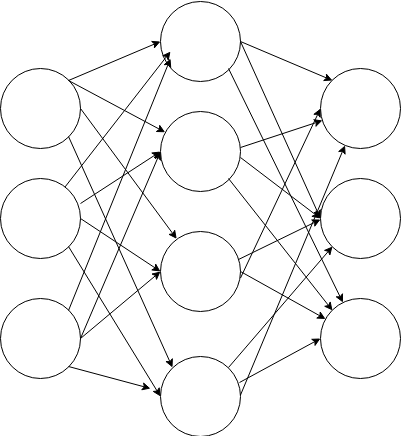
\includegraphics[height=10cm]{neural_net.png}
\subsubsection{General idea}
The general idea of machine learning with neural networks, is to make the computer think like a human; it is inspired by they way biological 
neural networks in the human brain process information \cite{neural_networks_0}. There are a lot of diffent neural networks, but all of them 
share the same underlying layer based architecture, where data is passed between layers where computation is done. The first layer is the input layer, 
which simply passes the data to the next layer, which is the hidden layers. The number of hidden layers is competely up to the model and the programmer, 
and this is where the intermediate processing/computation is done, before the data is passed to the output layer where we perform an activation function 
to define the output \cite{neural_networks_1}. 

If you have a lot of hidden layers in a neural network, we call it a \textit{deep} neural network. This 
is commonly used, and there is a lot of different deep networks with a lot of diffent use cases. To keep it simple for this thesis, I will explain one deep 
network called \textit{Recurrent Neural Network}. 

\subsubsection{Recurrent Neural Networks (RNN)}
This type of neural network is good for predicting something based on a sequence of data, like for example predicting words in a sentence, which 
can be especially useful for typing on a phone. Also doing predictions based on historical data, like a forecast, is something an RNN can do effectively, 
which the dataset I'm going to use in this thesis consist of. 

One downside to regular Recurrent Neural Networks, is that if the sequence of data is long, the prediction will most likely be off if something that was for example 
typed in the beginning of a long text is a dependancy for a prediction four chapters later, like the location of the main charater. The workaround for this
is something called \textit{Long Short-Term Memory Recurrent Neural Network (LSTM RNN)}, and is basically the idea of having additional logic to avoid 
the prediction model forgetting important facts.

\section{How can machine learning help people with bipolar disorder?}
The usage of machine learning in the medical fields is growing exponentially these days. There are so many use cases of machine learning, and of course 
it can help in the bipolar field too! Let's say bipolar patients had a device that measured their heart rate among other things 24 hours a day could 
feed the data into a machine learning model that could give the user live feedback on which bipolar state they are currently in. I think that would be very 
useful, for both the patients and doctors/nurses. Another use case coudl be if medical institutions could know in advance how many new bipolar patients to 
expect the next day. 

I believe that using machine learning in this field of study could help a lot of people get through their depression or mania, and potentially get rid 
of the condition competely.

\section{The dataset}
The dataset I will use in this project \cite{dataset} was collected for another study for motor activity in schizophrenia and major depression. 
Wit the data about schizophrenia stripped out, this dataset is sufficient for my thesis. It contains activity level data for 23 bipolar and unipolar patients, 
and 32 non-depressed contributors. From now on, I will refer to the bipolar/unipolar group as the \textit{condition group}, and the non-depressed group as 
the \textit{control group}. This is also done in the dataset details \cite{dataset_details}.

\section{What to do in this project}
My problem statement is "\problemStatement". This is an open project statement, which enables this project to contain both some classification and some regression.
To do this, I will use all the algorithms I have specified, beginning with the easiest ones (decision tree learning and random forest), before I try neural networks.

\section{Challenges and ethical concerns}
In most projects in the medical fields, there are going to be ethical concerns and challenges with privacy. What happens if someone that are not clearified for 
the data gets access to it? What if the database gets hacked? With new regulations (GDPR), privacy gets more and more important. However, in this project all
data is anonymized, and there will be no persons mentioned. 

\section{Related work}
List related work and discuss...

